%! Author = phili
%! Date = 28/06/2021

\section{Web Security}
\subsection{Introduction}
\begin{itemize}
    \item 56\% of internet traffic is automated (hacking tools etc.)
    \item Critical systems on the web
\end{itemize}
\subsection{OWASP}
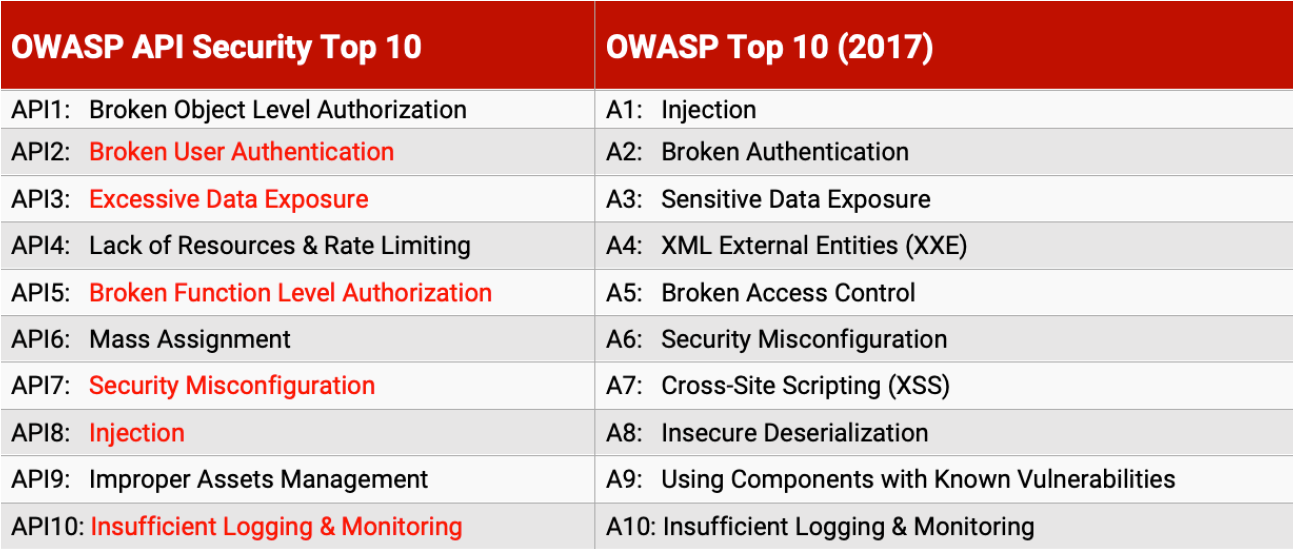
\includegraphics[width=\linewidth]{../img/owasp.png}

\subsection{Reasons for the many Security Incidents in the Web}
\begin{itemize}
    \item The way how we develop software (human errors)
    \item Almost no regulation
    \item Time to market (no time to update/fix/test)
    \item Not aware of the risk
    \item It's difficult
    \item Attractive for hackers, easy to access targets on the web
\end{itemize}

\subsection{XSS}
\begin{itemize}
    \item Client-side code injection attack (victim's browser)
    \item Executing malicious scripts in the victim's browser
    \item Vulnerable applications deliver malicious scripts
\end{itemize}
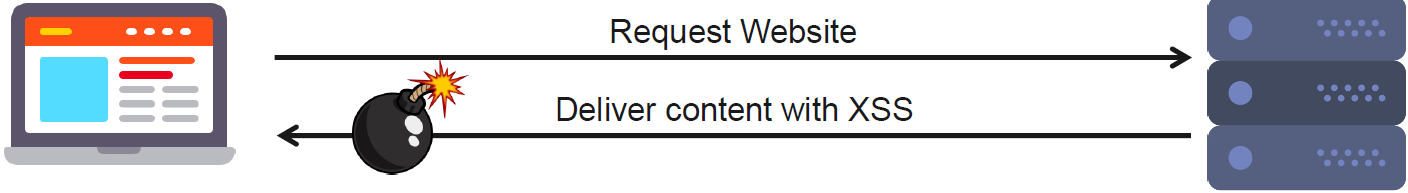
\includegraphics[width=0.7\linewidth]{../img/xss.pn.png}\\

\subsubsection{Stored XSS}
\begin{itemize}
    \item Script is permanently stored on the target server
    \item Malicious script is executed for every visitor
    \item \textbf{Typical Example:} Message board
\end{itemize}
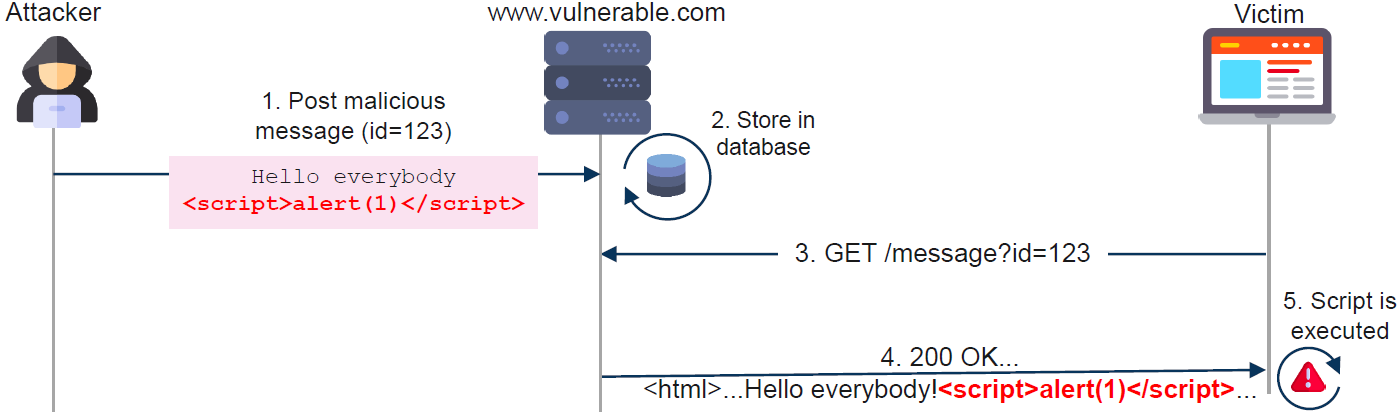
\includegraphics[width=\linewidth]{../img/xss_stored.png}
\textbf{Session Stealing Attack}\\
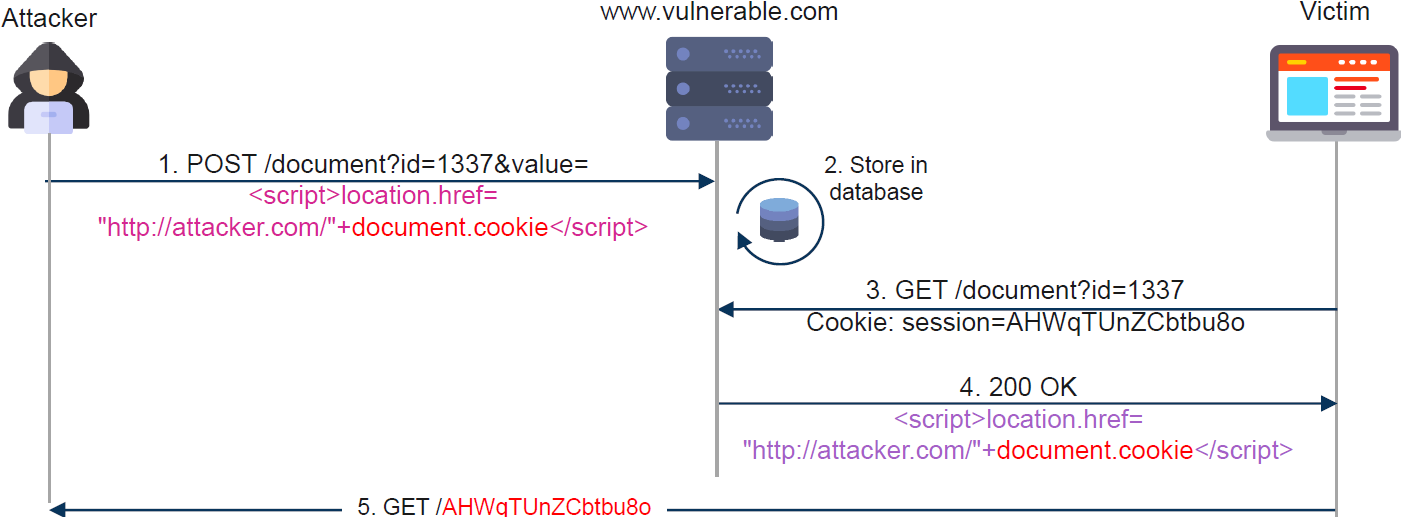
\includegraphics[width=\linewidth]{../img/xss_stored2.png}

\subsubsection{Reflected XSS}
\begin{itemize}
    \item Script is \textbf{not stored} on the target server
    \item Attacker usually needs to construct a malicious URL
    \item \textbf{Typical Example:} Search Form
\end{itemize}
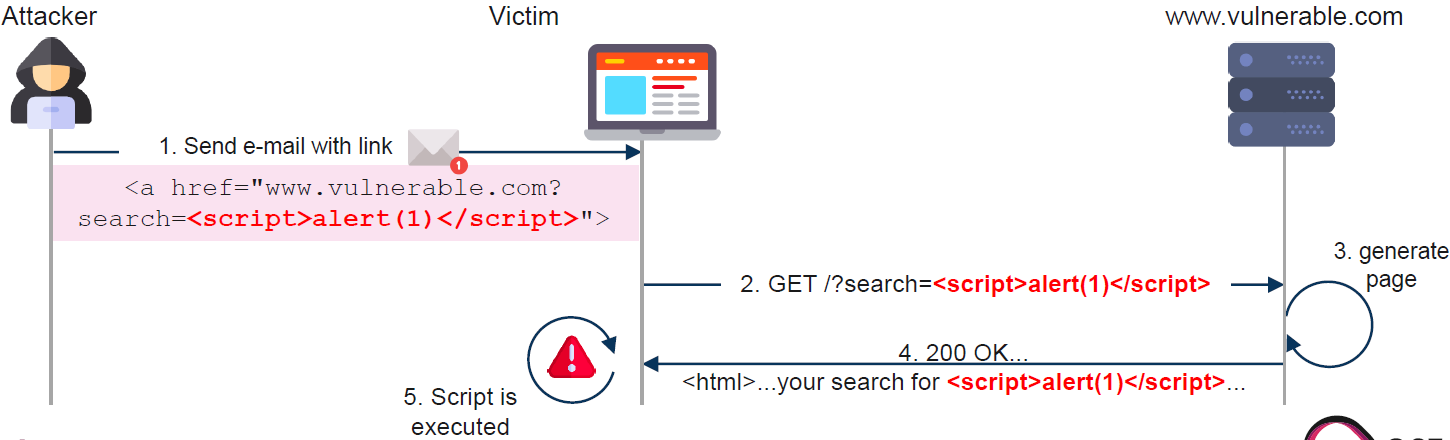
\includegraphics[width=\linewidth]{../img/xss_reflected.png}

\subsubsection{DOM based XSS}
\begin{itemize}
    \item Vulnerability is the client side code rather than server-side code
    \item Attacker needs to construct an URL
    \item Parameter of the URL is not processed by the server, but executed by the browser directly
\end{itemize}
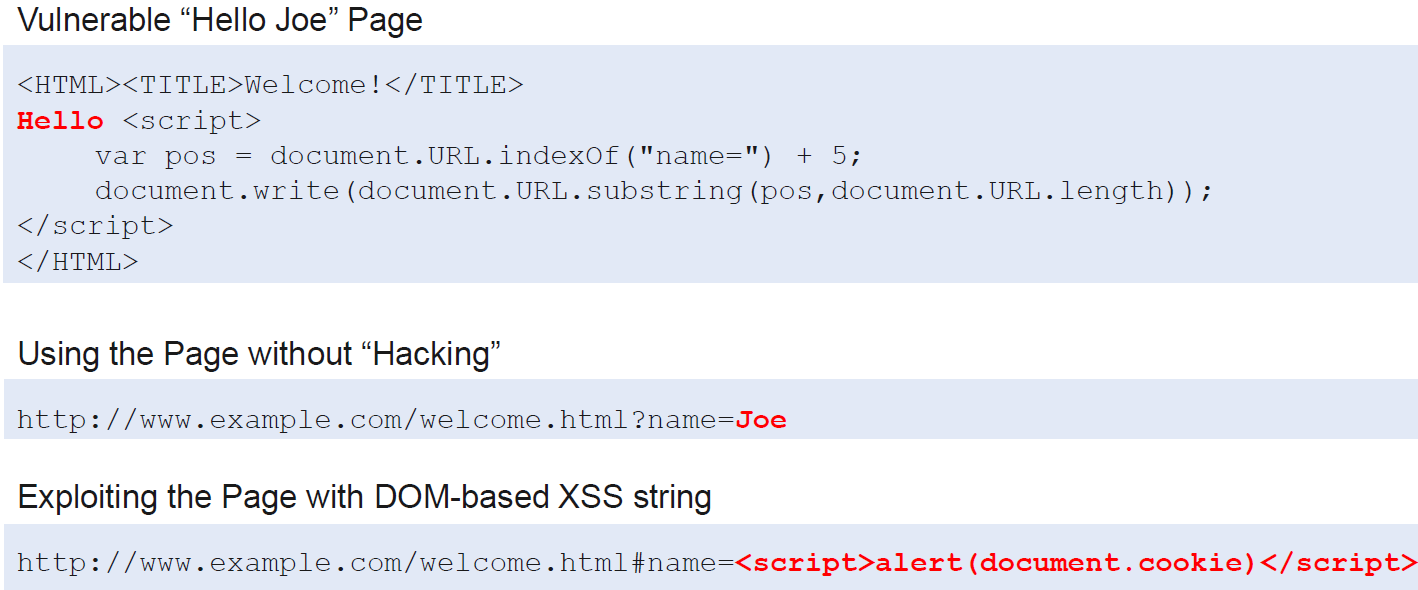
\includegraphics[width=\linewidth]{../img/xss_dom.png}

\subsubsection{Attack Vector Examples}
\begin{itemize}
    \item Script tags
    \item Event handler (\textit{onLoad, onClick} etc.)
    \item Links
    \item InnerHTML assignment (DOM-based XSS)
\end{itemize}

\subsubsection{Searching for XSS}
\begin{itemize}
    \item Play around with different strings in request params (script, \', \", etc.)
    \item In the page returned
    \begin{itemize}
        \item Search for the presence of test strings
        \item Check how the chars get filtered
        \item Find the problem and test with new strings
    \end{itemize}
\end{itemize}

\subsubsection{The power of \textless script src \textgreater}
\begin{itemize}
    \item Bypassing the SOP
\end{itemize}
\textbf{JavaScript from malware sites:}\\
JavaScript from www.attacker.com
IS \textbf{DENIED} from accessing resources
from www.vulnerable.com when the
JavaScript is loaded separately (e.g.
separate browser tab)\\
\textbf{Counter:}
JavaScript from www.attacker.com
IS \textbf{ALLOWED} to access resources
from www.vulnerable.com, if the
script is loaded by
www.vulnerable.com with
\textless script src="..."\textgreater

\subsubsection{XSS Protection}
\begin{itemize}
    \item Secure Programming
    \begin{itemize}
        \item Input / Output encoding of user supplied data (HTML entities)
        \item Input Validation (White/Blacklisting)
        \item Using XSS Protection Features in Frameworks
        \item Input sanitization of Web Frameworks
    \end{itemize}
    \item HTTP Response Header
    \item Cookie HttpOnly
    \begin{itemize}
        \item May prevent cookie / session stealing
        \item Malicious JavaScript can still \textbf{ride the session} and exfiltrate and manipulate the DOM
    \end{itemize}
    \item Browser XSS Filter (\textit{X-XSS-Protection: 1; mode=block})
    \begin{itemize}
        \item Asks Browser to render a blank page if XSS is detected
        \item Deprecated or never implemented for most browsers
        \item Poor detection rate
    \end{itemize}
    \item Content Security Policy (CSP)
    \begin{itemize}
        \item Firewall for the Browser
        \item Prevents code injection attacks like XSS
        \item Supported by modern browsers
        \item CSP defines, what is allowed to request from other domains
        \item CSP comes as http response header or HTML tag
    \end{itemize}
    \item Web Application Firewall
    \begin{itemize}
        \item WAF Input Validation
        \item Filtering HTTP Requests / Responses
        \item Searching for XSS Payload
    \end{itemize}
\end{itemize}

\subsection{Cross-Site Request Forgery}
\begin{itemize}
    \item End User executes unwanted actions while authenticated
\end{itemize}
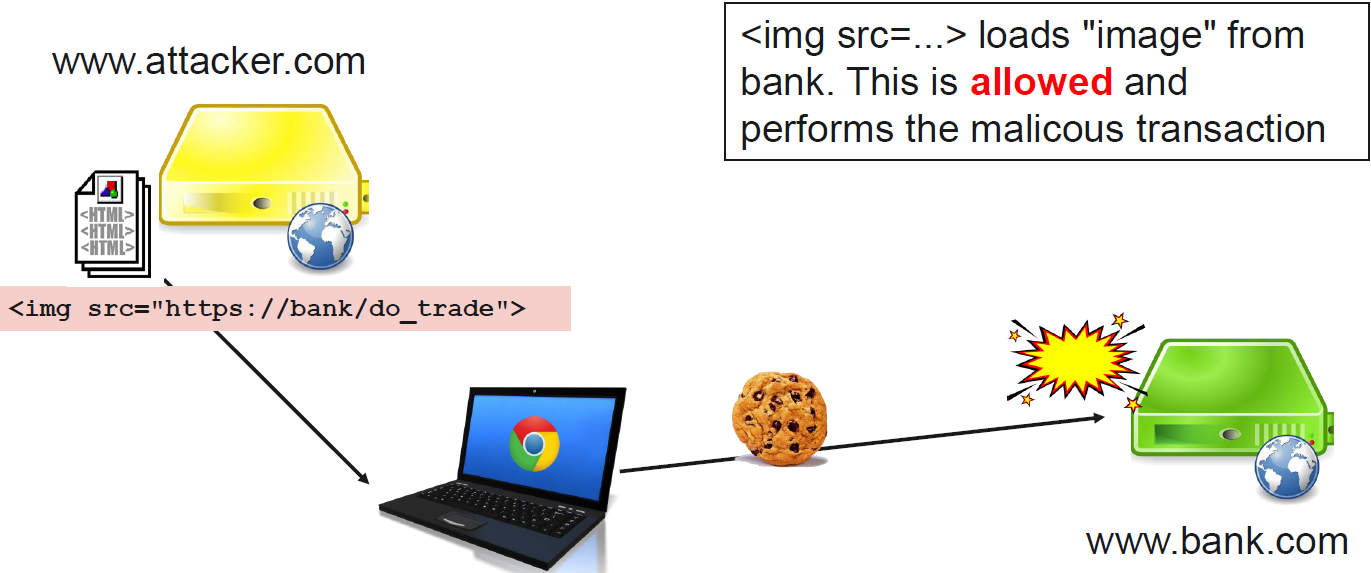
\includegraphics[width=\linewidth]{../img/xsrf.png}

\subsubsection{Pre-Requirement}
\begin{itemize}
    \item Know the target website / request
    \item Host the xsrf code somewhere
    \item Victim must have a valid session cookie
\end{itemize}

\subsubsection{XSRF Protection}
\begin{itemize}
    \item Random Token
    \begin{itemize}
        \item Form with a hidden field containing random token
    \end{itemize}
    \item SameSite Cookie Attribute
    \begin{itemize}
        \item Prevents browser from sending this cookie along with cross-site requests
        \item Mitigates cross-origin information leakage
        \item \textit{lax / strict}
    \end{itemize}
    \item CORS (only a mitigation)
    \begin{itemize}
        \item Configure CORS on the API service
        \item only allow requests from the fron-end origin
    \end{itemize}
    \item Framework Support
    \begin{itemize}
        \item AngularJS has built-in XSRF tokens on client side
        \item Server side must be implemented by the dev
    \end{itemize}
\end{itemize}

\subsection{HTTP Security Headers}
\textbf{Strict Transport Security}
\begin{itemize}
    \item HSTS
    \item \textit{Strict-Transport-Security: max-age=[ms]}
    \item Further requests in this time must occur over HTTPS
    \item Avoids all attacks based on HTTP downgrades
\end{itemize}
\textbf{X-Content-Type-Options}
\begin{itemize}
    \item nosniff
    \item Problem: Wrong Content-Type in HTTP Response
    \item e.g. Blocks a request if the requested type is \textit{style} and MIME type is not "text/css"
    \item Supported by all major browsers
\end{itemize}
\textbf{X-Frame-Options}
\begin{itemize}
    \item Prevent Website Framing
    \item Options: \textit{deny / SAMEORIGIN}
    \item Affects \textit{frame, iframe, embed, object}
\end{itemize}
\textbf{Referrer-Policy}
\begin{itemize}
    \item Control when URL information should be shared in the Referer header for other sites
    \item Options: \textit{no-referrer / same-origin / orign-when-cross-origin}
\end{itemize}
\textbf{Feature-Policy}
\begin{itemize}
    \item Allow and deny the use of browser features
\end{itemize}

\subsection{SQL Injection}
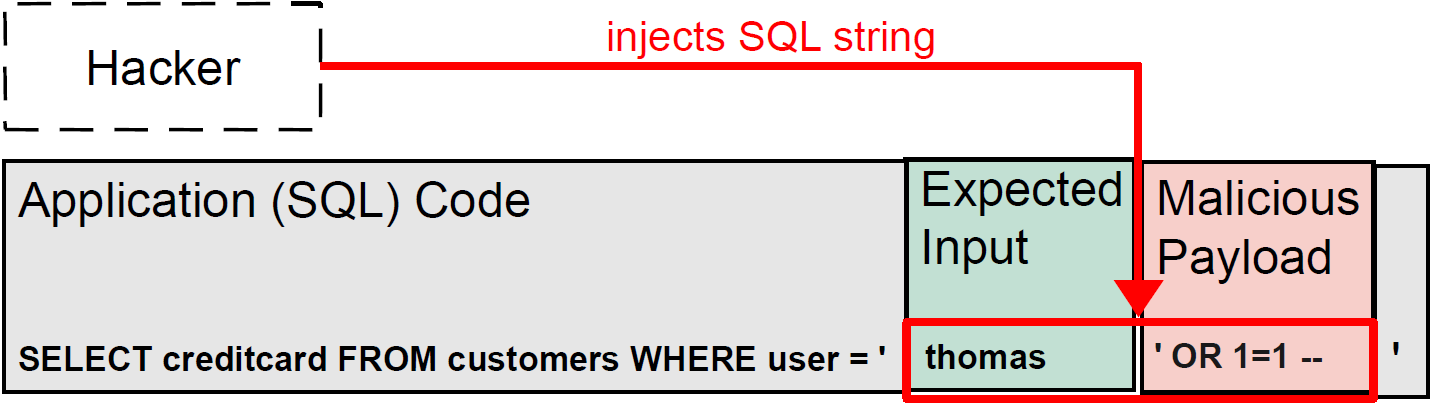
\includegraphics[width=\linewidth]{../img/sql_injection.png}
\subsubsection{Bypass Authentication}
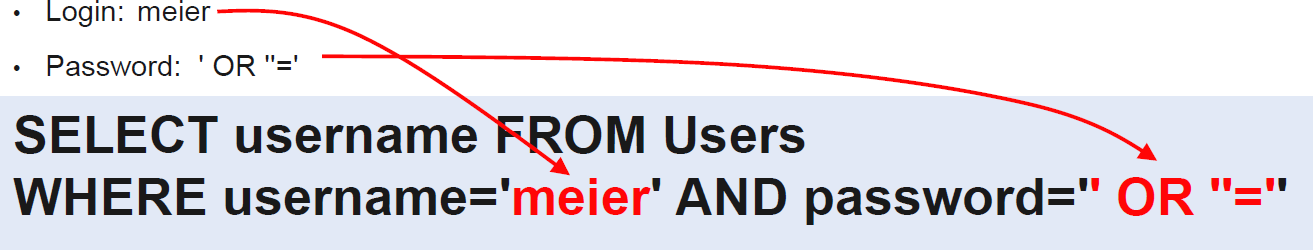
\includegraphics[width=\linewidth]{../img/sql_injection2.png}
\subsubsection{Fetch Arbitrary Information}
\begin{itemize}
    \item Access to System and catalog tables
\end{itemize}
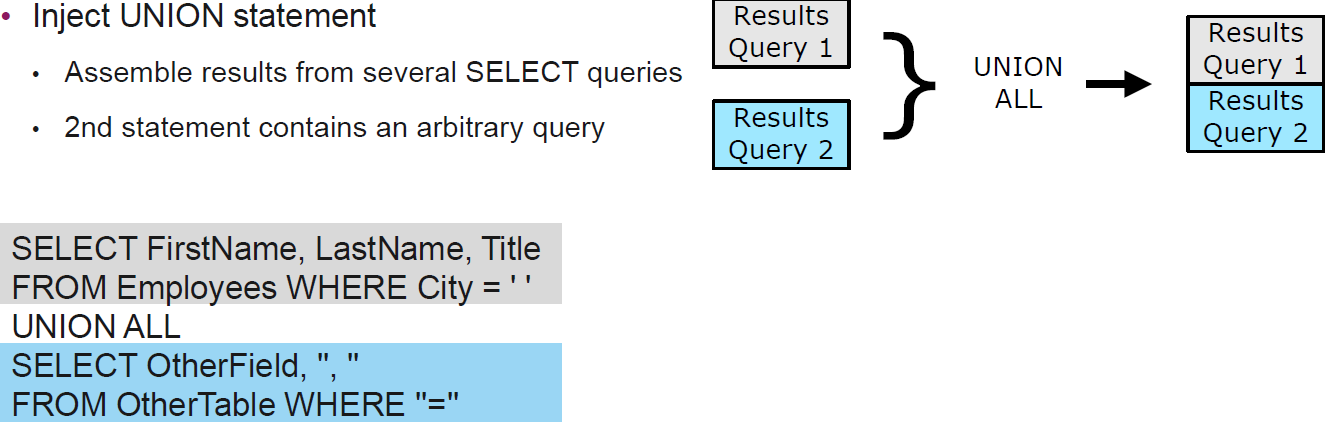
\includegraphics[width=\linewidth]{../img/sql_injection3.png}

\subsubsection{Hacking Database Example}
\begin{enumerate}
    \item What userID is running the MySQL database?
    \item Disclose Password hash from database
    \item Install Backdoor on Server through SQL Injection
    \item Upload more hacker tools on the server
\end{enumerate}

\subsubsection{Mitigation}
\begin{itemize}
    \item Secure Programming
    \begin{itemize}
        \item Prepared Statements / Stored Procedures
        \item Escaping
    \end{itemize}
    \item Error Handling
    \begin{itemize}
        \item Do not disclose details
    \end{itemize}
    \item Web Application Firewall
    \item DB least privileges
\end{itemize}

\subsection{XML External Entity Attack}
\subsubsection{XML Security}
\begin{itemize}
    \item XML signatures
    \item XML encryption
    \item XML key management
    \item Security Assertion Markup Language
    \item XML access control markup language
\end{itemize}

\subsubsection{Attack Vectors}
\textbf{XML Generator}\\
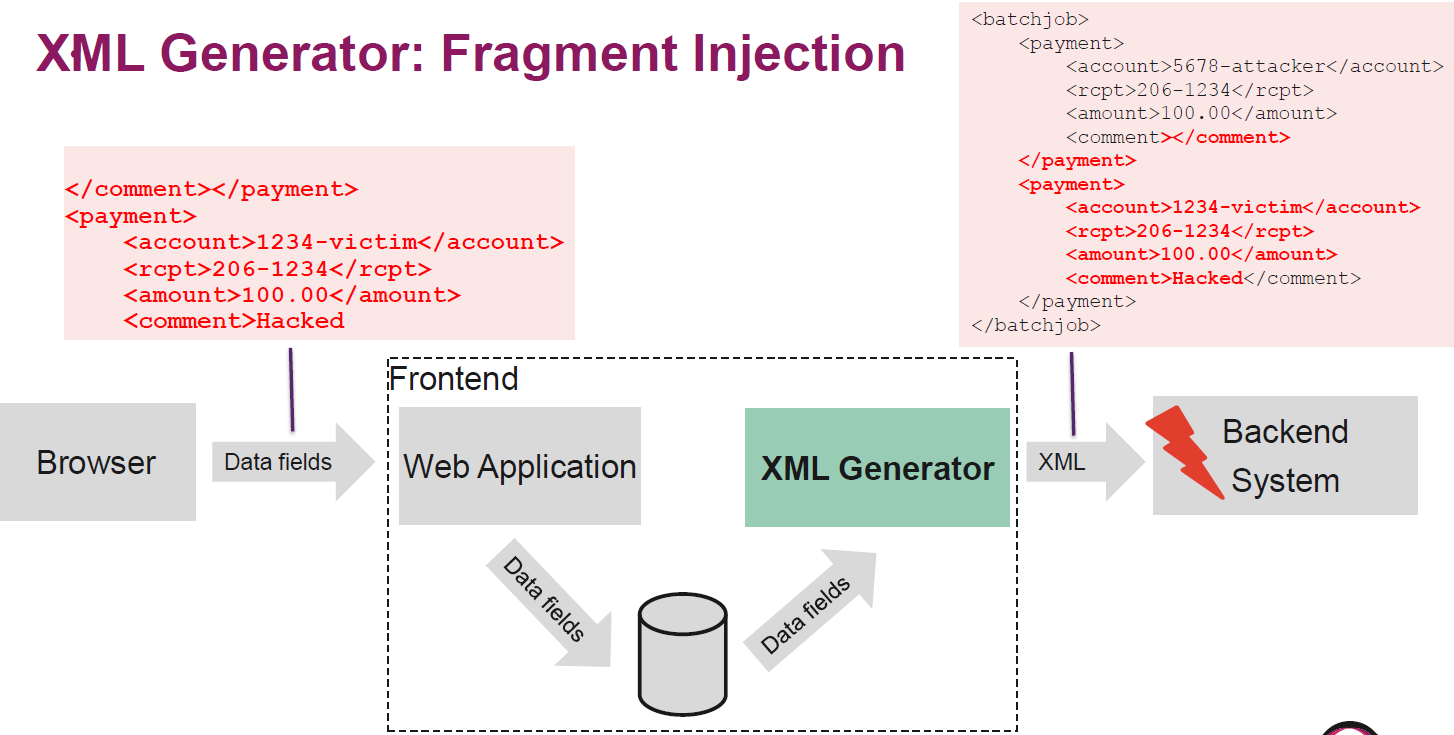
\includegraphics[width=\linewidth]{../img/xml_generator.png}
\textbf{Parser Attacks}
\begin{itemize}
    \item Attack Range
    \begin{itemize}
        \item DoS
        \item Inclusion of local files into XML documents (disclosure)
        \item Port scanning from the system where the parser is located
        \item Fetch data from local or remote systems
    \end{itemize}
\end{itemize}

\subsubsection{Mitigating XML Attacks}
\begin{itemize}
    \item Secure XML parser setup
\end{itemize}